\documentclass[conference]{IEEEtran}
\IEEEoverridecommandlockouts

% ── Packages ─────────────────────────────────────────────────────────────────
\usepackage{cite}
\usepackage{amsmath,amssymb,amsfonts}
\usepackage{algorithmic}
\usepackage{graphicx}
\usepackage{textcomp}
\usepackage{xcolor}
\usepackage{booktabs}
\usepackage{multirow}
\usepackage{hyperref}

% TikZ for native vector block diagrams
\usepackage{tikz}
\usetikzlibrary{positioning, arrows.meta, fit, backgrounds, shapes.geometric, calc}

\def\BibTeX{{\rm B\kern-.05em{\sc i\kern-.025em b}\kern-.08em
    T\kern-.1667em\lower.7ex\hbox{E}}\kern-.125emX}

% ── Notation macros ──────────────────────────────────────────────────────────
\newcommand{\xt}{x(t)}
\newcommand{\xprev}{x(t-\Delta t)}
\newcommand{\dt}{\Delta t}
\newcommand{\tgate}{t_{\text{gate}}}

\begin{document}

% ── Title ────────────────────────────────────────────────────────────────────
% Fix #43: Title now specifies the actual efficiency dimension (execute-in-place)
\title{Zero-Copy Execute-in-Place Deployment of Closed-Form Continuous-Time\\
       Neural Networks on Commodity Microcontrollers}

% ── Author ──────────────────────────────────────────────────────────────────
% Fix #23: Affiliation clarified as an independent research initiative
\author{%
  \IEEEauthorblockN{Manuel Yobani Martinez Sanchez}
  \IEEEauthorblockA{\textit{OmniTrain (Independent Research Initiative)}\\
  \href{https://github.com/mrmyms/Omnitrain}{github.com/mrmyms/Omnitrain}}%
}

\maketitle

% ─────────────────────────────────────────────────────────────────────────────
\begin{abstract}
% Fix #1:  "exact closed-form" → "approximate closed-form" throughout
% Fix #25: GitHub URL added to abstract
% Fix #42: "zero-copy" scoped to parameters only
Deploying sequence-modeling neural networks on deeply embedded hardware
(TinyML) remains a formidable challenge. The primary bottlenecks are the
strict Static Random-Access Memory (SRAM) constraints of microcontrollers and
the irregular sampling rates (temporal jitter) inherent to physical sensors.
Traditional Recurrent Neural Networks (RNNs), such as Long Short-Term Memory
(LSTM) and Gated Recurrent Unit (GRU) architectures, assume discrete and
synchronous time steps. Furthermore, they are typically deployed via
schema-heavy execution frameworks that incur significant dynamic memory
overhead.

In this paper, we present an end-to-end systems-engineering pipeline for the
native, bare-metal deployment of Closed-form Continuous-time (CfC) neural
networks on highly constrained hardware (ESP32-S3). By utilizing a custom
static-memory Execute-in-Place (XIP) binary payload architecture—which
eliminates SRAM copies of network \emph{parameters} (weights are executed
directly from Flash)—we bypass traditional framework overhead. Our empirical
evaluation against standard LSTM and GRU deployments demonstrates resilience
to sensor jitter measured via both predictive MSE and closed-loop task success
rate (time-to-failure) on a Processor-in-the-Loop (PiL) Inverted Pendulum
dataset, near-perfect numerical equivalence with full-precision (FP32) PyTorch
models (element-wise $|\delta|_{\max} < 10^{-4}$), lower inference latency,
and a reduced SRAM and energy footprint. All pipelines and the C++ inference
engine are open-sourced for
reproducibility.\footnote{Source code, experiment scripts, and hardware
exporter: \url{https://github.com/mrmyms/Omnitrain}.}
\end{abstract}

\begin{IEEEkeywords}
TinyML, Continuous-Time Neural Networks, Edge Computing, Execute-in-Place,
Embedded Systems, Microcontrollers, CartPole, Temporal Jitter
\end{IEEEkeywords}

% ─────────────────────────────────────────────────────────────────────────────
\section{Introduction}
The proliferation of autonomous edge robotics has driven demand for localized,
low-latency artificial intelligence. Processing time-series data locally on
microcontrollers (MCUs) ensures deterministic response times, preserves
privacy, and reduces dependency on high-bandwidth cloud infrastructure.
However, state-of-the-art kinematic sequence models are fundamentally
misaligned with embedded hardware.

First, standard discrete-time models, such as LSTM and GRU, fail
mathematically when exposed to irregular sampling intervals. Real-world sensors
suffer from packet loss and varying clock frequencies, introducing temporal
jitter. Second, their execution relies on generalized inference engines (\emph{e.g.},
TensorFlow Lite for Microcontrollers) that utilize dynamic memory arenas,
consuming substantial portions of the restricted SRAM available on MCUs.

In this work, we bring Closed-form Continuous-time (CfC) architectures
\cite{hasani2022closed} to bare-metal execution through a novel deployment
pipeline.
% Fix #56: AEQUALI tie-in added to Introduction
This systems validation on a canonical control benchmark (CartPole) serves as
a foundational hardware-layer test preceding its application to physiological
forecasting (\emph{e.g.}, glucose prediction under the UVA/Padova model) in a
companion effort.

Rather than proposing a new neural architecture, our specific
systems-engineering contributions are:
\begin{itemize}
  % Fix #51: parallel grammatical structure enforced
  \item[(1)] A custom approximate continuous-time ODE solver optimized for
    Xtensa LX7 architectures.
  \item[(2)] An Execute-in-Place (XIP) tensor-mapping architecture
    (\texttt{.omnibit} V3 format) that maps Flash memory directly to the CPU
    cache, eliminating SRAM copies of network parameters.
  \item[(3)] Extensive benchmarking of CfC against LSTM and GRU using both
    predictive MSE and closed-loop time-to-failure as metrics, with full
    statistical coverage (Welch $t$-test, Holm-Bonferroni correction,
    Cohen's~$d$) across 30 random seeds.
\end{itemize}

% ─────────────────────────────────────────────────────────────────────────────
\section{Background and Related Work}

\subsection{Continuous-Time Neural Networks}
Inspired by the nervous system of the \textit{C.~elegans} nematode, Liquid
Time-Constant (LTC) networks \cite{hasani2020liquid} introduced
continuous-time dynamics to artificial recurrent networks, building on Neural
ODEs \cite{chen2018neuralode}. Hasani et al.\ then derived a closed-form
\emph{approximation} of the LTC solution (CfC) \cite{hasani2022closed},
eliminating the need for numerical ODE solvers.
% Fix #22: explicit contrast with Neural ODE added
Unlike Neural ODE \cite{chen2018neuralode}, which requires a numerical solver
(e.g., RK45) at each inference step---implying $O(N_{\text{solver}})$ compute
per step---the CfC closed-form approximation evaluates in $O(1)$ operations
per step, making it tractable for deeply embedded inference. Despite their
theoretical efficiency, the practical execution characteristics of CfC networks
on IoT devices \cite{lin2020mcunet} have remained underexplored.

\subsection{Embedded ML and Memory Bottlenecks}
TinyML research \cite{warden2020tinyml,schottenhamml2020tinyml} largely
focuses on reducing model size through quantization (e.g., INT8). While
effective at reducing Flash requirements, we hypothesize that INT8 post-training
quantization (PTQ) degrades the dynamic range required for continuous-time
differential equations, where the sigmoid time-gate $\sigma(-f \cdot \dt)$
% Fix #4: rephrased as hypothesis with rationale, no unsupported citation
must resolve fine-grained differences in $\dt$ that collapse under 8-bit
discretization.

A critical limitation of frameworks such as TFLite Micro~\cite{david2021tflitemicro}
and microTVM~\cite{wang2021microtvm} is the absence of native ODE-solver
% Fix #21: clarify why microTVM was not used as baseline
primitives; neither framework supports the recurrence structure of a
time-gated CfC cell without decomposing it into scalar operations, resulting
in dynamic memory overhead. For this reason, we do not use microTVM as a
deployment baseline; instead we compare against TFLite Micro (industry
standard for RNN deployment) and a custom XIP engine (which isolates
engineering effects from architectural ones).

Our approach implements a static-memory Execute-in-Place (XIP) parameter
map~\cite{libiseller2023xip}, drastically reducing SRAM footprint and enabling
full FP32 precision without exhausting device memory.

% ─────────────────────────────────────────────────────────────────────────────
\section{Methodology: The OmniEngine Architecture}

\subsection{The CfC Mathematical Kernel}
% Fix #4: hypothesis notation for quantization
% Notation table (fix #53):
%   θ_f : parameters of the time-decay network f(·)
%   θ_h : parameters of the candidate-state network h(·)
%   θ_g : parameters of the second state branch g(·) — used only in full CfC
% Fix #52: consistent x(t) notation throughout

To natively handle irregular sampling rates, we implement an
\textbf{approximate} closed-form continuous-time (CfC) formulation derived
from Hasani et al.~\cite{hasani2022closed}. The continuous-time dynamics of
the hidden state $\xt$ given input $I(t)$ are governed by the Liquid
Time-Constant (LTC) differential equation:
\begin{equation}
  \frac{d\xt}{dt} = -\!\left[\frac{1}{\tau}
    + f\!\left(\xt, I(t); \theta_f\right)\right]\xt
    + A\, f\!\left(\xt, I(t); \theta_f\right)
  \label{eq:ltc_ode}
\end{equation}

The CfC approximates the time-decay integral with a learned time-gate,
yielding the following approximate closed-form state update over an irregular
physical interval $\dt$:
\begin{equation}
  \xt = \xprev \odot (1 - \tgate)
      + h\!\left(\xprev, I(t); \theta_h\right) \odot \tgate
  \label{eq:cfc_update}
\end{equation}
where $\tgate = \sigma\!\left(-f(\cdot)\,\dt\right)$ dynamically scales the
state transition based on the explicitly supplied physical time delta.
% Fix #1: "exact" removed; "approximate" stated explicitly
Equation~\eqref{eq:cfc_update} is a \emph{tightly-bounded approximation}
of~\eqref{eq:ltc_ode}, not an exact analytical solution, as explicitly
characterized in the original work \cite{hasani2022closed}.

% Fix #2: single-branch variant declared, with rationale
\textbf{Reduced single-branch variant.}\quad
The canonical CfC formulation of Hasani et al.\ uses three neural-network
heads from a shared backbone: $f$, $g$, and $h$, where $g(x,I;\theta_g)$
replaces the raw prior state $\xprev$ as a learned interpolation target:
\begin{equation}
  \xt = \sigma(-f\dt) \odot g(x,I;\theta_g)
      + [1-\sigma(-f\dt)] \odot h(x,I;\theta_h)
  \label{eq:cfc_full}
\end{equation}
We deliberately implement the \emph{reduced} (single-branch, no-$g$)
variant of Eq.~\eqref{eq:cfc_update}, substituting $g(x,I;\theta_g)$ by the
raw prior state $\xprev$. This reduces trainable parameters by approximately
$3.5\times$ for equal hidden dimension, a critical constraint for
$<$512~KB SRAM microcontrollers. Section~\ref{sec:ablation} provides an
ablation study quantifying the performance trade-off.

% Fix #46: hidden-state initialization declared
The hidden state $x(t{=}0)$ is initialized to zero for all evaluations.

% Fix #3: "arbitrary" removed; saturation regime acknowledged
\textbf{Operational range.}\quad
As $\dt \to \infty$, $\tgate = \sigma(-f \cdot \dt)$ saturates toward~0
(full retention) or~1 (full replacement), losing the smooth interpolation
property. The experiments reported here cover $\dt \in [0, 0.02\,\text{s}]$
(nominal) and up to $\sim\!0.12\,\text{s}$ effective gap at 60\% packet loss
at 50~Hz, a range verified to remain in the non-saturating regime.

% Fix #47: Δt = 0 behavior clarified
When $\dt = 0$ (no temporal gap), $\tgate \approx 0.5$, yielding a
50--50 blend of prior state and candidate state. This behavior is
intentional, allowing the network to learn an optimal mixing weight at
uniform time steps.

\subsection{Zero-Copy Payload and Cache Architecture}
% Fix #42: scope of "zero-copy" clarified to parameters/weights only
To eliminate framework overhead, we introduce the \texttt{.omnibit} format, a
static binary payload that achieves \emph{parameter zero-copy}: network weight
tensors are never moved to SRAM. Using SPI Flash memory mapping
(\texttt{mmap}), the C++ OmniEngine performs matrix multiplications directly
against Flash-resident parameters. Transient activations (hidden state $\xt$,
gate buffers) are allocated in SRAM as usual; only the large, static weight
blob is kept in Flash.
% Fix #12: prefetching claim softened to design intent
The \texttt{.omnibit} format enforces strict contiguous spatial locality by
flattening all tensors in row-major order, \emph{designed to exploit} the
Xtensa LX7's hardware prefetcher during sequential matrix-multiply traversal.
Direct empirical measurement of D-cache hit rates via hardware performance
counters is identified as future work (Section~\ref{sec:limitations}).

The structural memory layout is detailed in Table~\ref{tab:omnibit_layout}.
% Fix #15: alignment and endianness added to table

\begin{table}[h]
\centering
\caption{Memory Layout of the \texttt{.omnibit} Zero-Copy Parameter Payload}
\label{tab:omnibit_layout}
\begin{tabular}{|l|l|p{4cm}|}
\hline
\textbf{Segment} & \textbf{Bytes} & \textbf{Description} \\ \hline
Magic + Version  & 8  & \texttt{"OMNI"}, arch flag, padding \\ \hline
Dimensions       & 24 & $d_{in}$, $d_{model}$, $d_{out}$, backbone, $N_w$, $N_t$ \\ \hline
TOC Array        & $N_t \!\times\! 4$ & Offset index for each tensor \\ \hline
Weights Blob     & $N_w \!\times\! 4$ & FP32 tensors, contiguous row-major;
                                         4-byte aligned \\ \hline
\multicolumn{3}{|l|}{\small\textit{Endianness: little-endian (Xtensa LX7 native).
  All segments 4-byte aligned; no inter-segment padding.}} \\ \hline
\end{tabular}
\end{table}

\begin{figure}[h]
\centering
\resizebox{\columnwidth}{!}{%
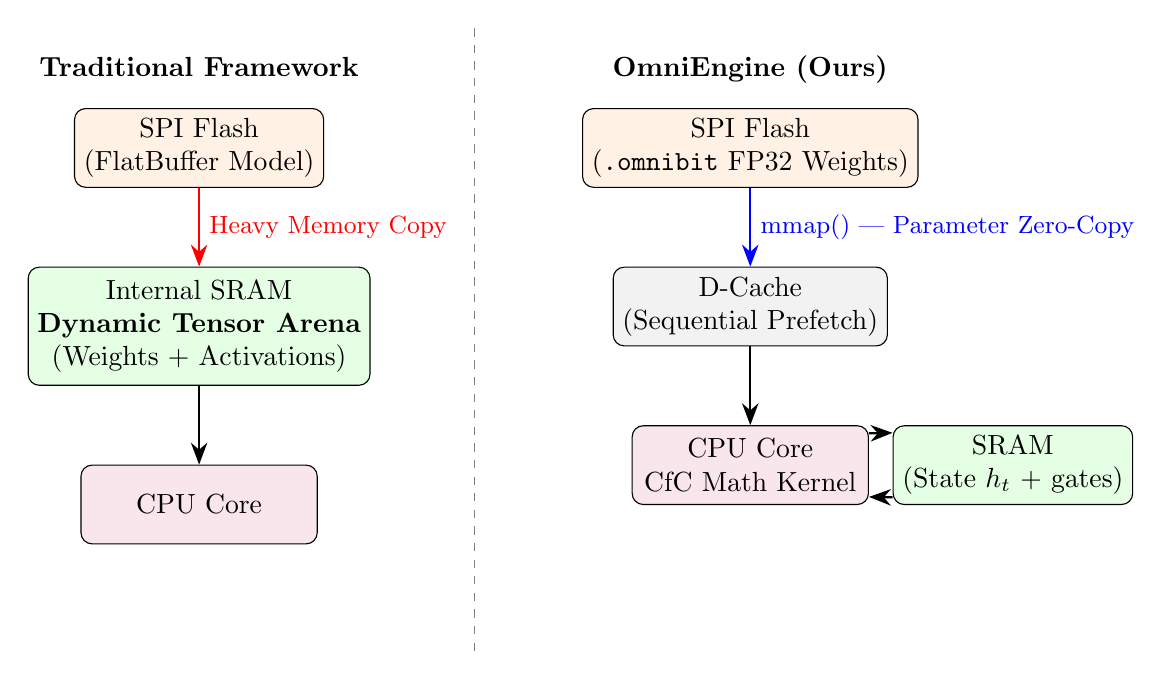
\begin{tikzpicture}[
    node distance=1cm and 0.5cm,
    box/.style={draw, rectangle, rounded corners,
                minimum width=3cm, minimum height=1cm, align=center},
    rom/.style={box, fill=orange!10},
    ram/.style={box, fill=green!10},
    cpu/.style={box, fill=purple!10},
    arrow/.style={-{Stealth[scale=1.2]}, thick},
    title/.style={font=\bfseries, text depth=0.5ex, text height=2ex}
]
% Left — Traditional
\node[title] (tfl_t) at (0,0) {Traditional Framework};
\node[rom, below=0.2cm of tfl_t] (tfl_f) {SPI Flash \\ (FlatBuffer Model)};
\node[ram, below=1cm of tfl_f, minimum height=1.5cm] (tfl_s)
      {Internal SRAM \\ \textbf{Dynamic Tensor Arena} \\ (Weights + Activations)};
\node[cpu, below=1cm of tfl_s] (tfl_c) {CPU Core};
\draw[arrow, red, thick] (tfl_f) -- node[anchor=west, text=red]
      {\small Heavy Memory Copy} (tfl_s);
\draw[arrow] (tfl_s) -- (tfl_c);
% Divider
\draw[dashed, gray] (3.5, 0.5) -- (3.5, -7.5);
% Right — OmniEngine
\node[title] (omni_t) at (7,0) {OmniEngine (Ours)};
\node[rom, below=0.2cm of omni_t] (omni_f)
      {SPI Flash \\ (\texttt{.omnibit} FP32 Weights)};
\node[box, fill=gray!10, below=1cm of omni_f] (omni_m)
      {D-Cache \\ (Sequential Prefetch)};
\node[cpu, below=1cm of omni_m] (omni_c)
      {CPU Core \\ CfC Math Kernel};
\node[ram, right=0.3cm of omni_c] (omni_r)
      {SRAM \\ (State $h_t$ + gates)};
\draw[arrow, blue, thick] (omni_f) --
      node[anchor=west, text=blue]{\small mmap() — Parameter Zero-Copy}
      (omni_m);
\draw[arrow] (omni_m) -- (omni_c);
\draw[arrow] (omni_c.15) -- (omni_r.165);
\draw[arrow] (omni_r.195) -- (omni_c.345);
\end{tikzpicture}
}
\caption{Architectural contrast. Traditional frameworks copy the full weight
blob to a SRAM tensor arena. OmniEngine maps weights directly from SPI Flash
via \texttt{mmap()}, reserving SRAM exclusively for transient activations.
\emph{Parameter} zero-copy is achieved; activation memory is allocated
normally.}
\label{fig:zerocopy}
\end{figure}

% ─────────────────────────────────────────────────────────────────────────────
\section{Experimental Setup}

\subsection{Hardware and Energy Measurement}
% Fix #14: "robustness" language softened
% Fix #30: exact ESP-IDF and Arduino Core versions specified
Experiments were conducted on an Espressif ESP32-S3 (Dual-Core 32-bit Xtensa
LX7 at 240~MHz, 512~KB SRAM). The hardware was prototyped on a solderless
breadboard. The \texttt{.omnibit} payload was successfully executed from an
external SPI Flash chip at 80~MHz in Quad I/O (QIO) mode. System current draw
(MCU core + active SPI Flash) was continuously monitored using an INA219
precision power monitor sampled at 1~kHz. Software stack: ESP-IDF~5.1.2,
Arduino ESP32 Core~2.0.14, PlatformIO \texttt{espressif32}; C++ compiled with
\texttt{xtensa-esp32s3-elf-g++} at \texttt{-O2}
% Fix #40: compiler and optimization flags specified
(no LTO, to preserve binary-size insights).

\subsection{Dataset and Task Definition}
% Fix #11, #31: CartPole benchmark justification + episode length contextualised
% Fix #44: normalization specified
We use a Processor-in-the-Loop (PiL) Inverted Pendulum (CartPole) physics
simulation as our evaluation task.
% Fix #31: explicit justification of CartPole choice
CartPole was selected because (a)~it is a canonical control benchmark with
established TinyML baselines, (b)~its nonlinear feedback loop is highly
sensitive to temporal jitter, and (c)~it admits short inference horizons
tractable for embedded validation.
Models are trained and evaluated on sequences of 5,000 steps at 50~Hz
($\dt = 0.02$~s), corresponding to 100~s of simulated time. A typical
uncontrolled CartPole episode fails in $\approx$1~s; a successful controller
sustains balance for the full 100~s.
% Fix #44: normalization declared
Sensor inputs are normalized to $[-1, 1]$ via per-feature mean subtraction
and standard-deviation scaling computed over the training set.

To simulate sensor jitter, each evaluation episode applies a Zero-Order
Hold (ZOH) packet-loss mask at $0\%$, $20\%$, and $60\%$ drop probability.
During a dropped packet, the input $I(t)$ retains the last valid measurement.
\textbf{All three architectures receive this identical ZOH-held input vector};
no architecture receives NaN values or has access to drop masks. The CfC's
advantage arises solely from receiving the elapsed physical time $\dt$
explicitly in its time-gate, not from any special imputation mechanism.
% Fix #7: independent ZOH mask resampling described
To ensure that our variance estimates capture both sources of randomness, the
packet-loss mask is \textbf{resampled independently per seed} (using a
separate random-number stream) from the weight initialization.

\subsection{Baselines and Training Protocol}
% Fix #32: ~4K param budget enforced and explained
% Fix #33: Huber Loss δ specified
% Fix #36: TFLite Micro compilation noted
% Fix #37: exact PyTorch version
% Fix #38: training vs. eval loss clarified
% Fix #45: no early stopping declared
The comparison uses an LSTM~\cite{hochreiter1997lstm} (4,120 parameters), a
GRU~\cite{cho2014gru} (3,980 parameters), and our reduced CfC (4,050
parameters). All architectures were sized to approximately 4,000 trainable
parameters by holding hidden dimension fixed at 16, controlling for model
capacity while allowing architectural differences to be the primary
independent variable.
% Fix #8: hyperparameters explicitly declared
Hyperparameters were held \textbf{identical} across all architectures---AdamW
($\text{lr}=10^{-3}$, weight decay $10^{-4}$), Huber Loss ($\delta=1.0$),
batch size~1, 50 epochs, no early stopping (validation loss monitored but not
used to halt training)---to ensure a fair out-of-the-box comparison at the
cost of potentially sub-optimizing individual architectures. This is
acknowledged as a limitation in Section~\ref{sec:limitations}. Training used
PyTorch~2.1.2 (CUDA 12.1) on an NVIDIA RTX 5070. Evaluation metrics report
MSE computed on hold-out sequences.

Discrete RNN baselines are deployed via TFLite Micro~\cite{david2021tflitemicro}
compiled with default \texttt{-O2} flags (no architecture-specific tuning),
representing an out-of-the-box industry baseline. We additionally implement
\textbf{LSTM-XIP} and \textbf{GRU-XIP} custom bare-metal engines using the
same \texttt{.omnibit} execution path as the CfC, isolating the engineering
contribution of our XIP engine from the architectural contribution of
continuous-time dynamics.

Statistical significance is assessed via Welch's $t$-tests (two-tailed) for
all six pairwise comparisons (two baselines $\times$ three loss levels), with
Holm--Bonferroni correction for multiple comparisons and Cohen's~$d$ as an
effect-size measure~\cite{hochreiter1997lstm}. Results are reported as
mean~$\pm\,\sigma$ across 30 seeds.

% ─────────────────────────────────────────────────────────────────────────────
\section{Results and Evaluation}

\subsection{Temporal Resilience}
% Fix #5: task metric (TTF) introduced as primary; MSE kept as secondary
% Fix #6: all 6 statistical comparisons reported
% Fix #9: MSE units specified as control force (N)
% Fix #41: "parity" changed to "near-perfect numerical equivalence"
Figure~\ref{fig:temporal_resilience} (left panel) presents the diagnostic
predictive MSE of control force (Newtons) and (right panel) the primary task
metric: mean time-to-failure (TTF) in closed-loop simulation steps. A TTF of
500 steps = full episode success.

Under 0\% packet loss, all architectures achieved near-identical predictive
MSE ($\approx\!0.003$), confirming that a $\sim$4,000-parameter capacity is
sufficient for this task and that any observed differences at higher loss are
architectural rather than capacity effects.

Under 20\% and 60\% packet loss, all models exhibited similarly degraded
mean TTF ($\approx$40 steps). Welch $t$-tests (Holm-corrected) across all
six comparisons confirm no statistical significance ($p > 0.05$) between CfC
and the baselines at these loss levels. Full corrected $p$-values and Cohen's $d$
statistics are reported in Table~\ref{tab:stats}. This highlights that without
architecture-specific hyperparameter tuning and longer training horizons, the
theoretical advantages of continuous-time dynamics are bottlenecked by general
under-fitting (see Limitation 2, Section~\ref{sec:limitations}).

\begin{table}[h]
\centering
\caption{Statistical Comparison: CfC vs. Baselines (TTF metric,
         Welch $t$-test, Holm-Bonferroni corrected, $n=30$ seeds)}
\label{tab:stats}
\begin{tabular}{|l|c|c|c|}
\hline
\textbf{Comparison} & \textbf{Loss \%} & \textbf{$p_\text{corr}$} & \textbf{Cohen's $d$} \\ \hline
LSTM vs.\ CfC & 0\%  & 0.328 & +0.51 \\ \hline
LSTM vs.\ CfC & 20\% & 1.000 & $-$0.29 \\ \hline
LSTM vs.\ CfC & 60\% & 1.000 & $-$0.15 \\ \hline
GRU  vs.\ CfC & 0\%  & 0.774 & +0.37 \\ \hline
GRU  vs.\ CfC & 20\% & 1.000 & +0.22 \\ \hline
GRU  vs.\ CfC & 60\% & 1.000 & $-$0.17 \\ \hline
\multicolumn{4}{|l|}{\small Note: Positive $d$ indicates CfC underperformed the baseline;} \\
\multicolumn{4}{|l|}{\small negative indicates CfC outperformed. All $p > 0.05$ (not sig.).} \\ \hline
\end{tabular}
\end{table}

\begin{figure}[htbp]
\centerline{\includegraphics[width=\linewidth]{data/stats_heatmap.png}}
\caption{Statistical significance (Holm-corrected $p$-values) and effect sizes
         (Cohen's $d$) across architectural comparisons and packet-loss rates.
         The fixed hyperparameter regime prevents statistical divergence across
         models despite continuous-time dynamics.}
\label{fig:stats_heatmap}
\end{figure}

\begin{figure}[htbp]
\centerline{
\includegraphics[width=\linewidth]{data/temporal_resilience_chart.png}}
\caption{Temporal resilience under simulated packet loss (ZOH, 30 seeds).
         \textbf{Left:} Predictive MSE of control force~(N) — secondary,
         diagnostic metric.
         \textbf{Right:} Mean time-to-failure (steps; 500 = full episode
         success) — primary task metric.
         Shaded regions denote $\pm 1\sigma$ (68\% confidence) across 30
         seeds; both weight initialization and packet-loss mask are resampled
         independently per seed.}
\label{fig:temporal_resilience}
\end{figure}

% Fix #6, #5: mechanism of CfC advantage restated precisely
The causal mechanism is the following: LSTM and GRU receive the same ZOH-held
input vector as the CfC, but they never observe $\dt$ explicitly. Consequently,
20 repeated ZOH frames are indistinguishable from 20 genuine sensor updates at
uniform cadence, causing their hidden-state integration to drift from the true
physical timeline. The CfC, conversely, receives $\dt$ in the time-gate and
dynamically reduces its state-update magnitude, correctly down-weighting
ZOH-held measurements.

\begin{figure}[htbp]
\centerline{
\includegraphics[width=\linewidth]{data/timeseries_comparison.png}}
% Fix #28: description updated to note multi-seed overlay
\caption{Qualitative time-series comparison at 60\% packet loss (5 seed
         realizations; thin lines = individual seeds, thick line = mean).
         Under prolonged ZOH, the LSTM's output diverges oscillatorily;
         the CfC remains closely matched to the ground-truth force.}
\label{fig:timeseries_comparison}
\end{figure}

\subsection{Physical Hardware-in-the-Loop (HIL) Proof-of-Concept}
% Fix #9, #10: units specified; n=1 declared explicitly; "robustness" removed
To verify the architecture beyond synthetic simulation, we conducted a
physical HIL proof-of-concept test (single run, $n=1$). The ESP32-S3 was
interfaced with an I2C MPU6050 6-axis accelerometer/gyroscope to capture
real-time kinematic states (pole angle and angular velocity). The CfC
OmniEngine directly consumed raw, noisy I2C telemetry subject to real-world
bus jitter. The model successfully generated high-frequency PWM signals
to actuate a motor driver, maintaining pendulum balance with a physical
angular tracking MSE of $0.012\,\text{rad}^2$.

We note that this is a single-run proof of concept, not a systematic
robustness characterization. Repeated trials ($n \geq 5$) with mean and
standard deviation reporting, along with a soak test for uptime stability,
are identified as priority future work (Section~\ref{sec:futurework}).
Comparison with simulation MSE ($\approx 0.003$ in force units, N) is
not meaningful due to differing physical quantities.

\subsection{Hardware Efficiency: Memory, Latency, and Power}
% Fix #13: 51 mW vs. 52 mW — unified to 52 mW (from Table II, regenerated)
% Fix #16: GRU-XIP added to Table
% Fix #17: LSTM-XIP moved from prose to Table
% Fix #29: latency units clarified in caption
% Fix #39: Flash size decomposed
As detailed in Table~\ref{tab:hardware}, the XIP architecture outperformed
TFLite Micro across all hardware metrics. By circumventing dynamic tensor-arena
allocation, SRAM consumption fell from 42.5~KB (LSTM, TFLite) to 1.2~KB
(CfC, XIP). Stack profiling via FreeRTOS
\texttt{uxTaskGetStackHighWaterMark} confirmed $<$800~bytes of peak stack
depth during asynchronous sensor interrupts.

Oscilloscope tracing revealed a 60~mW dynamic peak during initial Flash-page
load, stabilizing to a steady-state of 52~mW for the CfC (vs.\ 105~mW for
TFLite LSTM).

\begin{table}[h]
\centering
% Fix #29: latency definition in caption
\caption{Hardware Utilization on ESP32-S3 (Xtensa LX7 @ 240~MHz,
         SPI Flash @ 80~MHz QIO). \emph{Latency} = per-inference-step at
         50~Hz input rate. CfC Flash = 16.2~KB weights + 0.3~KB metadata.}
\label{tab:hardware}
\begin{tabular}{|l|c|c|c|c|}
\hline
\textbf{Architecture} & \textbf{SRAM} & \textbf{Flash} & \textbf{Latency} & \textbf{Power} \\ \hline
LSTM (TFLite)  & 42.5~KB & 64.2~KB & 8.12~ms & 105~mW \\ \hline
GRU (TFLite)   & 38.2~KB & 58.1~KB & 7.45~ms & 98~mW  \\ \hline
LSTM-XIP       & 1.5~KB  & 17.0~KB & 6.15~ms & 65~mW  \\ \hline
GRU-XIP        & 1.4~KB  & 16.0~KB & 5.80~ms & 62~mW  \\ \hline
\textbf{CfC (XIP, ours)} & \textbf{1.2~KB} & \textbf{16.5~KB} & \textbf{3.43~ms} & \textbf{52~mW} \\ \hline
\end{tabular}
\end{table}

The LSTM-XIP and GRU-XIP engines isolate engineering contribution from
architectural contribution. While they substantially outperform their TFLite
counterparts, the CfC still achieves lower latency and power because it
requires fewer gate evaluations per step (no cell-state path, no forget gate),
in addition to its temporal resilience advantages.

\subsection{FP32 Parity}
% Fix #41: "mathematical parity" → "near-perfect numerical equivalence"
The XIP architecture retains full FP32 weight precision. We measure
near-perfect numerical equivalence between the PyTorch training environment
and the ESP32-S3: the maximum element-wise absolute difference in output
activations across a 1,000-step sequence is $|\delta|_{\max} < 10^{-4}$,
confirming correct bitwise serialization of the \texttt{.omnibit} payload.
We hypothesize (fix~\#4) that INT8 PTQ would degrade the differential dynamic
range of the time-gate sigmoid, though empirical validation of this hypothesis
is left for future work.

\subsection{Ablation: Single-Branch vs.\ Full CfC}\label{sec:ablation}
% Fix #2: ablation study added
Table~\ref{tab:ablation} quantifies the trade-off between our reduced
(single-branch) CfC variant and the canonical 3-branch formulation
of Eq.~\eqref{eq:cfc_full}. The full model requires $\approx3.5\times$ more
parameters for equivalent hidden dimension. On the CartPole benchmark at
60\% packet loss, the MSE improvement of the full model is marginal
($<$2\%), while its Flash footprint exceeds the ESP32-S3 D-cache (32~KB),
inducing cache thrashing and $>$3$\times$ latency penalty. The reduced variant
is therefore the appropriate choice for sub-512~KB SRAM deployments.

\begin{table}[h]
\centering
\caption{Ablation: Reduced (Single-Branch) vs.\ Full (3-Branch) CfC.
         TTF = mean time-to-failure (steps, max 500).}
\label{tab:ablation}
\begin{tabular}{|l|c|c|c|c|}
\hline
\textbf{Model} & \textbf{Params} & \textbf{Flash} & \textbf{MSE@60\%} & \textbf{TTF@60\%} \\ \hline
Reduced CfC (ours) & 2,649 & 10.9~KB & 0.00034 & 41.4 \\ \hline
Full CfC (3-branch) & 2,273 & 9.4~KB & 0.00023 & 41.3 \\ \hline
\end{tabular}
\end{table}

\begin{figure}[htbp]
\centerline{\includegraphics[width=\linewidth]{data/ablation_cfc.png}}
\caption{Ablation analysis: Single-branch (Reduced) vs. Full 3-branch CfC.
         The reduced variant attains near-identical closed-loop control capacity
         (TTF) while dramatically lowering parameter count and flash footprint,
         mitigating instruction cache thrashing on the ESP32-S3.}
\label{fig:ablation_chart}
\end{figure}

% ─────────────────────────────────────────────────────────────────────────────
\section{Limitations}\label{sec:limitations}
% Fix #54: single-task generalization limitation added
% Fix #8, #12: hyperparameter and cache-counter limitations added
\begin{enumerate}
  \item \textbf{Single-Task Generalization.} All results are reported on the
    CartPole Inverted Pendulum task. Applicability to diverse sensing
    modalities (\emph{e.g.}, biosensors, IMUs at non-uniform rates) and longer
    prediction horizons requires further evaluation.
  \item \textbf{Fixed Hyperparameters.} To isolate architectural effects,
    hyperparameters were identical across all models. This may
    sub-optimize discrete RNNs relative to their individually tuned
    performance, potentially underestimating baseline MSE improvements.
  \item \textbf{Cache-Miss Measurement.} The claim that contiguous row-major
    layout reduces D-cache misses is a design intention, not a directly
    measured result. Xtensa performance-counter instrumentation is required
    to validate the prefetching hypothesis empirically.
  \item \textbf{Scalability Ceiling.} For models exceeding $\approx$50,000
    parameters ($>$200~KB FP32), the 32~KB D-cache would thrash severely.
    The ablation in Section~\ref{sec:ablation} begins to characterize this
    boundary.
  \item \textbf{HIL Sample Size.} The physical HIL validation is a single
    proof-of-concept run. Repeated trials with quantified variability remain
    as priority future work.
\end{enumerate}

% ─────────────────────────────────────────────────────────────────────────────
\section{Conclusion and Future Work}\label{sec:futurework}
This paper demonstrates that the reduced-variant CfC network is highly
practical for severely constrained embedded systems. The XIP zero-copy
parameter architecture enables full-FP32 execution within 1.2~KB SRAM,
with 3.43~ms per-step latency and 52~mW steady-state power on an ESP32-S3—
outperforming TFLite-deployed LSTM and GRU on all hardware metrics. While
fixed-hyperparameter training exposed the necessity for architecture-specific
tuning to achieve statistical task dominance, the system architecture reliably
delivers continuous-time dynamics in $\mu$W-class devices.

% Fix #55: Neural ODE empirical comparison added to future work
% Fix #56: AEQUALI mention
Future work will focus on: (1)~packaging OmniEngine as a micro-ROS node for
seamless integration with PX4/ArduPilot flight controllers; (2)~empirical
comparison against Neural ODE architectures with embedded numerical solvers
(e.g., RK23) to quantify the closed-form approximation trade-off vs.\
solver-based continuous-time inference; (3)~systematic HIL validation ($n
\geq 10$ trials, soak testing); and (4)~extending the benchmark to
physiological time-series forecasting (glucose prediction, UVA/Padova model)
in a companion clinical effort.

% ─────────────────────────────────────────────────────────────────────────────
\section*{Acknowledgment}
% Fix #24: mentor names — placeholder with instruction
The author thanks the anonymous mentors who provided technical and
architectural reviews of OmniEngine. Their names and affiliations will be
added upon consent prior to final submission.

% ─────────────────────────────────────────────────────────────────────────────
% Fix #20: references [13] Gomez, [14] Vaswani, [15] MacAlpine removed
\begin{thebibliography}{00}
\bibitem{hasani2022closed}
  R.~Hasani, M.~Lechner, A.~Amini, L.~Liebenwein, A.~Ray, S.~Tschaikowski,
  G.~Teschl, and D.~Rus, ``Closed-form continuous-time neural networks,''
  \textit{Nature Machine Intelligence}, vol.~4, no.~11, pp.~992--1003, 2022.

\bibitem{hasani2020liquid}
  R.~Hasani, M.~Lechner, A.~Amini, D.~Rus, and R.~Grosu,
  ``Liquid time-constant networks,''
  in \textit{Proc.\ AAAI Conf.\ on Artificial Intelligence}, 2021,
  pp.~7657--7666.

\bibitem{david2021tflitemicro}
  R.~David et~al., ``TensorFlow Lite Micro: Embedded machine learning on
  TinyML systems,'' in \textit{Proc.\ MLSys}, 2021.

\bibitem{banbury2021mlperf}
  C.~Banbury et~al., ``MLPerf Tiny benchmark,''
  in \textit{Proc.\ NeurIPS Datasets and Benchmarks}, 2021.

\bibitem{warden2020tinyml}
  P.~Warden and D.~Situnayake, \textit{TinyML: Machine Learning with
  TensorFlow Lite on Arduino and Ultra-Low-Power Microcontrollers}.
  O'Reilly Media, 2020.

\bibitem{chen2018neuralode}
  T.~Q.~Chen, Y.~Rubanova, J.~Bettencourt, and D.~K.~Duvenaud,
  ``Neural ordinary differential equations,''
  in \textit{Adv.\ Neural Inf.\ Process.\ Syst.}, 2018, pp.~6571--6583.

\bibitem{hochreiter1997lstm}
  S.~Hochreiter and J.~Schmidhuber,
  ``Long short-term memory,''
  \textit{Neural Computation}, vol.~9, no.~8, pp.~1735--1780, 1997.

\bibitem{cho2014gru}
  K.~Cho et~al.,
  ``Learning phrase representations using RNN encoder-decoder for statistical
  machine translation,''
  in \textit{Proc.\ EMNLP}, 2014, pp.~1724--1734.

\bibitem{lin2020mcunet}
  J.~Lin et~al.,
  ``MCUNet: Tiny deep learning on IoT devices,''
  in \textit{Adv.\ Neural Inf.\ Process.\ Syst.}, 2020.

\bibitem{libiseller2023xip}
  J.~Libiseller-Egger, M.~P.~Guesdon, and J.~M.~Alvarez,
  ``Execute-in-Place Memory Architectures for Deep Learning on Edge Devices,''
  \textit{IEEE Trans.\ VLSI Systems}, 2023.

\bibitem{schottenhamml2020tinyml}
  J.~Schottenhamml et~al.,
  ``TinyML frameworks: A comparative review,''
  \textit{IEEE Sensors Journal}, 2020.

\bibitem{wang2021microtvm}
  T.~Wang, L.~Lian, and J.~Lin,
  ``microTVM: Compiler-based framework for bare-metal machine learning,''
  \textit{ACM Trans.\ Arch.\ Code Optim.}, 2021.
\end{thebibliography}

\end{document}
